\documentclass[paper=a4, fontsize=11pt]{scrartcl} % A4 paper and 11pt font size
\usepackage[T1]{fontenc}  % proper encoding for output file
\usepackage[utf8]{inputenc}  % except UTF-8 character in source
\usepackage[english]{babel}  % set document language
\usepackage{amsmath,amsfonts,amsthm}  % math type setting
\usepackage{mhchem}  % chemical expressions
\usepackage{graphicx}  % inclue graphics
\usepackage{url}
\usepackage{caption}
\usepackage{subcaption}
\setlength\parindent{0pt} % Removes all indentation from paragraphs

% Macro to conveniently typeset chemical symbols.
\newcommand{\symb}[1]{$\,\mathrm{#1}$}


\title{Exercise 3: Line shape}
\author{Sample Solution}
\date{Effective: 25.11.2016}

%%%%%%%%%%%%%%%%%%%%%%%%%%%%%%%%%%%%%%%%%%%%%%%%%%%%%%%%%%%%%%%%%%%%%%%%%%%%%%%
\begin{document}

\maketitle

1. Choose an individual line and perform calculations over a restricted 
frequency range for a number of different pressures. Keep the temperature and 
constituent mixing ratio constant.

\begin{itemize}
  \item How does the shape of the spectral lines change?
    \begin{itemize}
      \item Figure~\ref{fig:abs_xsec} shows the absorption cross-section around 
      the 183\,GHz water-vapor line. With increasing pressure the lines become
      more narrow but also stronger.
    \end{itemize}
\end{itemize}
\vfill
\begin{figure}[h!]
  \centering
  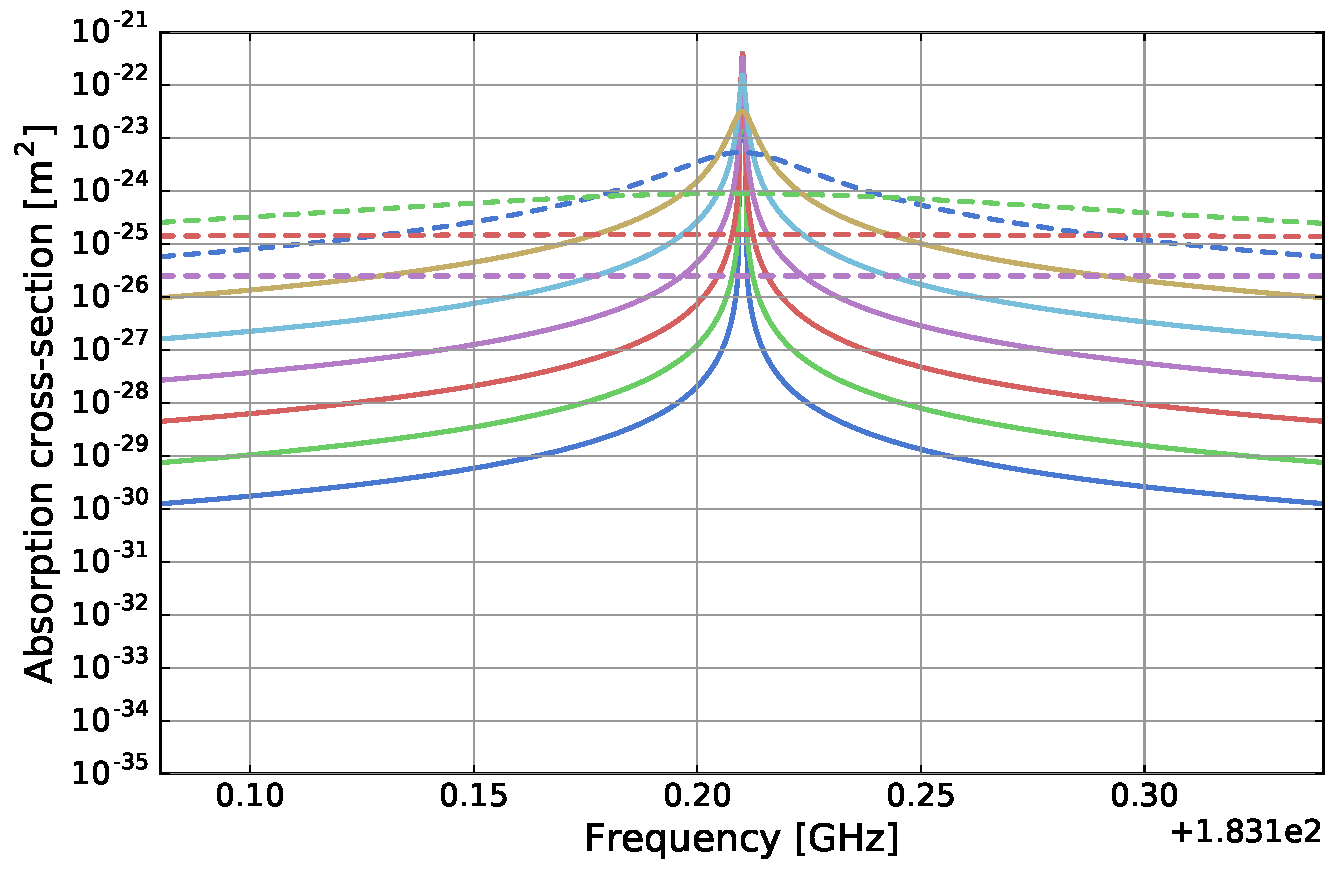
\includegraphics[width=0.9\textwidth]{plots/line_center_crosssection.pdf}
  \caption{Absorption cross section $\sigma$ for $H_2O$ at different pressures.}
  \label{fig:abs_xsec}
\end{figure}

\clearpage
By now we investigated absorption in terms of the absorption cross-section 
$\sigma$. Another widely used unit is the absorption coefficient $\alpha$. It 
takes the number concentration $n$ of the absorber into account.

\begin{itemize}
  \item How does the absorption coefficient in the line centre change, if 
pressure is changed?
    \begin{itemize}
      \item Figure~\ref{fig:abs_coeff} shows the absorption coefficient. It is 
      the product of $\sigma$ and the amount of absorbing molecules per cubic meter 
      $n$. The absorption lines also widen with increasing pressure, but the 
      absorption coefficient in the line center is constant.
    \end{itemize}
\end{itemize}
\vfill
\begin{figure}[h!]
  \centering
  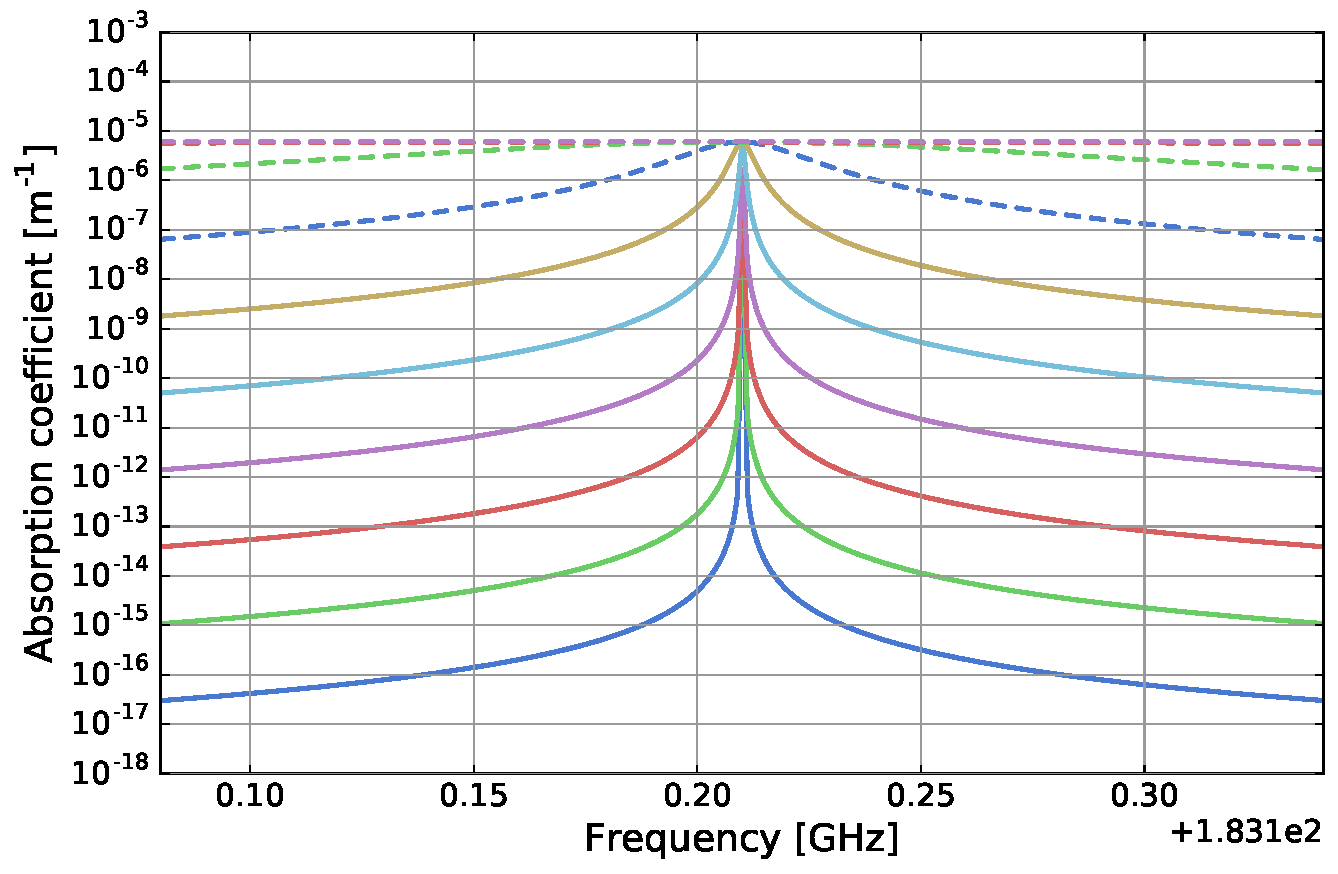
\includegraphics[width=0.9\textwidth]{plots/line_center.pdf}
  \caption{Absorption coefficient $\alpha$ for $H_2O$ at different pressures.}
  \label{fig:abs_coeff}
\end{figure}

\clearpage
2. A measure of the line width is the full-width at half maximum. Make a plot of 
this as a function of altitude (pressure). Do this for a microwave line and an 
infrared line.\\

Figure~\ref{fig:mw_linewidth} shows the linewidth at different pressures for a 
microwave line. Figure~\ref{fig:ir_linewidth} shows the same quanitites for an 
infrared line. Both plots show two dominant regimes: a pressure depending 
behaviour at high pressures and a constant linewidth at low pressures. The 
transition between both regimes differs for both spectra regions. This can be 
explained by different mechanisms of lineshapes.

Figure~\ref{fig:lineshapes} shows the curves for three different lineshape 
models: Lorentz, Doppler and Voigt-Kuntz. The Lorentz model is purely 
temperature depending and therefore constant in our setup. Lorentz describes a 
linear dependency between lineshape and atmospheric pressure. Voigt-Kuntz is a 
combination of both models with a transition for pressures in between. The 
Doppler model is frequency depending and therefore more relevant for infrared 
lines.
\vfill
\begin{figure}[ht]
  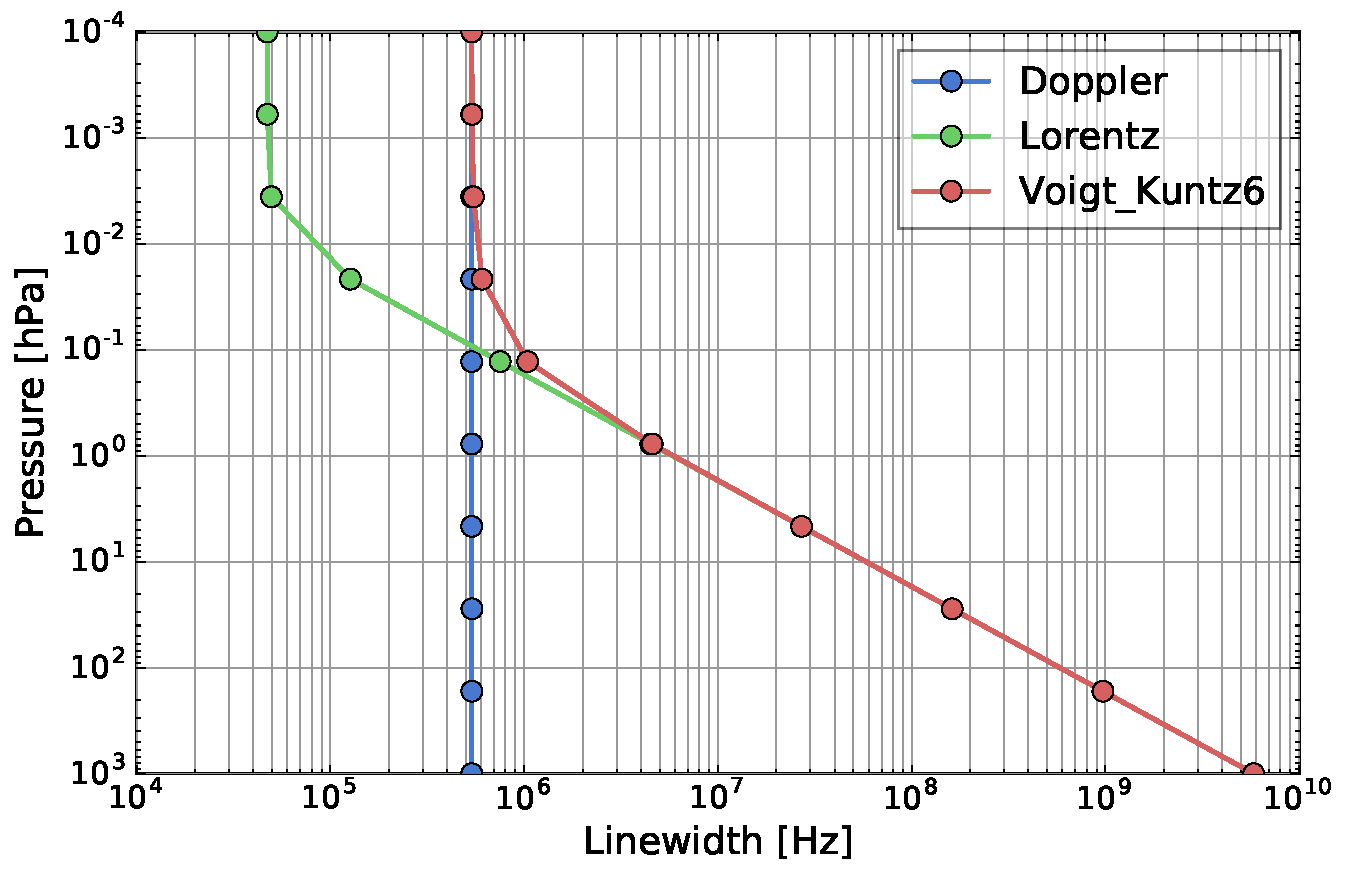
\includegraphics[width=0.9\textwidth]{plots/linewidth.pdf}
  \caption{Linewidth at different pressures with constant temperature.
  Different lineshapes are used: Doppler (blue), Lorentz (green)
  and Voigt-Kuntz (red).}
  \label{fig:lineshapes}
\end{figure}

\begin{figure}[ht]
  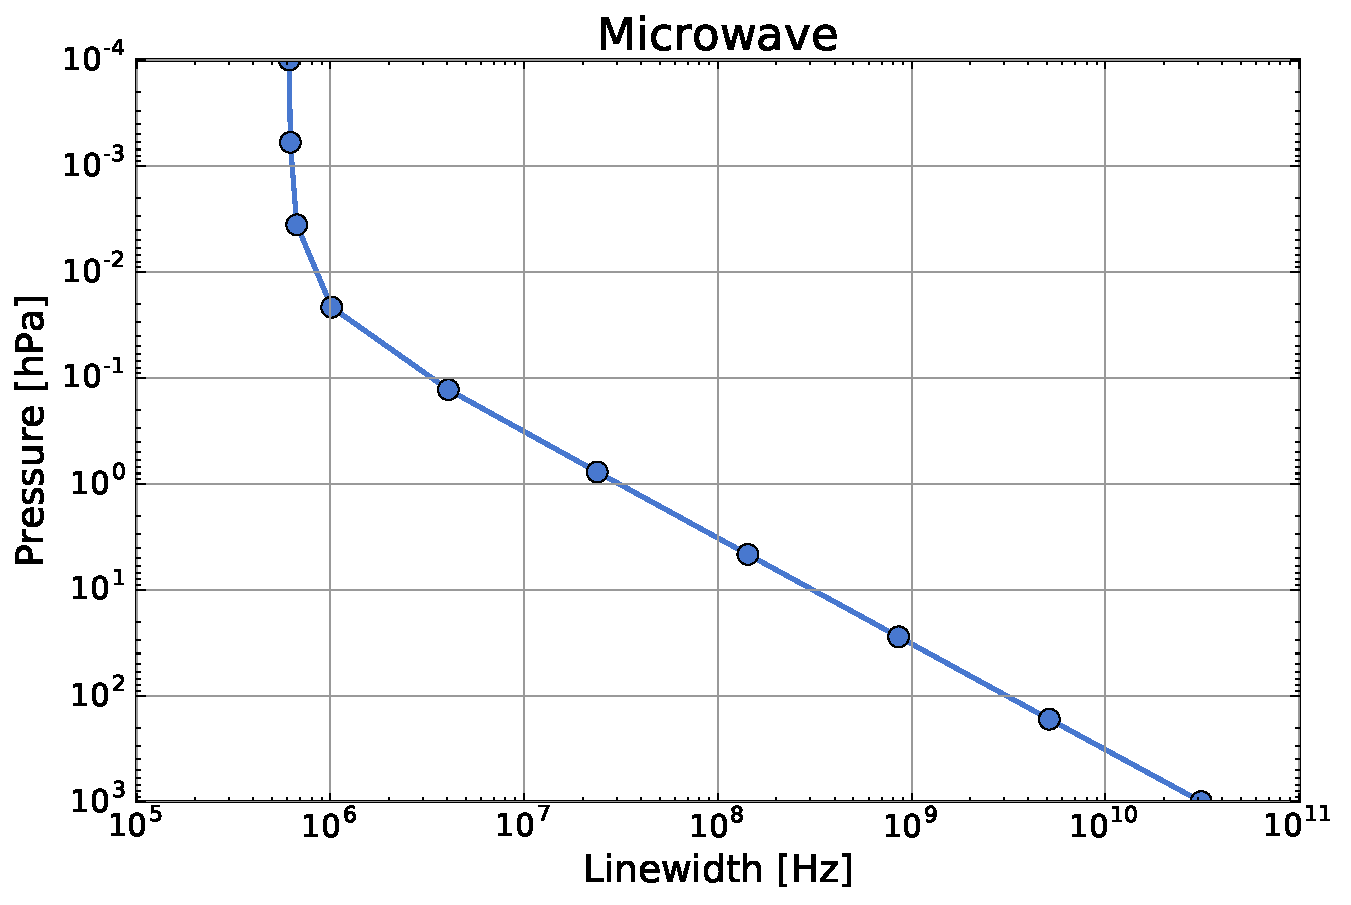
\includegraphics[width=0.9\textwidth]{plots/mw_linewidth.pdf}
  \caption{Linewidth of a microwave line ($H_2O$) at different pressures.}
  \label{fig:mw_linewidth}
\end{figure}

\begin{figure}[ht]
  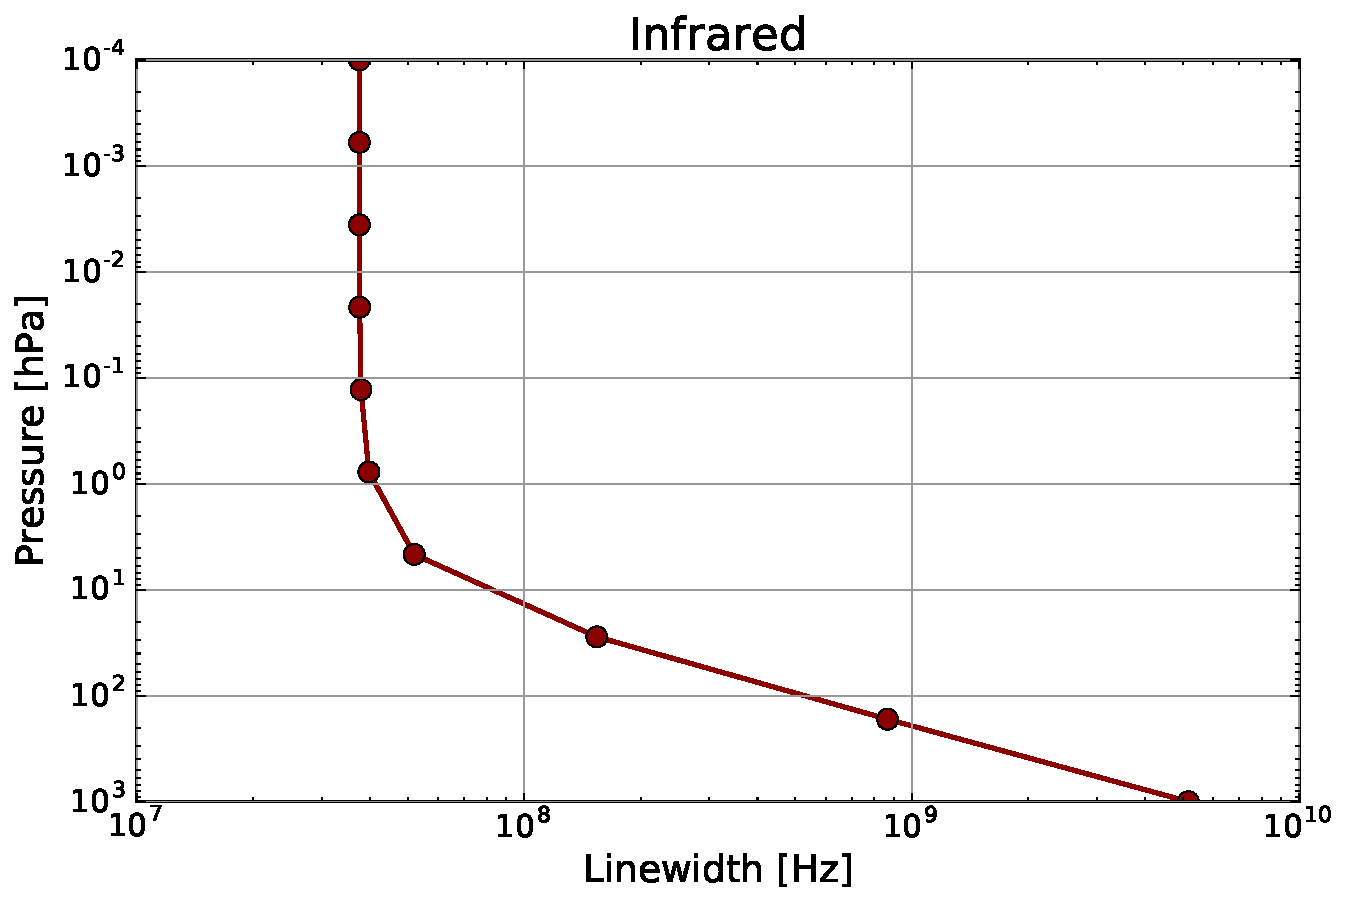
\includegraphics[width=0.9\textwidth]{plots/ir_linewidth.pdf}
  \caption{Linewidth of a infrared line ($CO_2$) at different pressures.}
  \label{fig:ir_linewidth}
\end{figure}
\end{document}